\documentclass{article}
\usepackage{fancyhdr}
\usepackage{titlesec}
\usepackage{graphicx}
\graphicspath{ {./img/} }
\usepackage{multirow}
\usepackage[hidelinks]{hyperref}

\pagestyle{fancy}
\fancyhf{}
\lhead{Modul 9 Praktikum Jaringan Komputer}
\rfoot{\footnotesize Page \thepage}
\lfoot{\footnotesize Mahyus Ihsan, S.Si, M.Si \newline Jurusan Informatika Universitas Syiah Kuala \newline Modul oleh : Diky Wahyudi, Furqan Al Ghifari, Rendika Rahmaturrizki}
\renewcommand{\headrulewidth}{1pt}
\renewcommand{\footrulewidth}{1pt}

\titleformat*{\section}{\small\bfseries}

\begin{document}
    \begin{center}
        \textbf{Modul 9 Praktikum Jaringan Komputer}

        \textbf{MikroTik}
    \end{center}

    \section*{Deskripsi Singkat}
	\begin{flushleft}
		Mikrotik merupakan sistem operasi berupa perangkat lunak yang digunakan untuk menjadikan komputer menjadi router jaringan.
		Sistem operasi ini sangat cocok untuk keperluan administrasi jaringan komputer, misalnya untuk membangun sistem jaringan komputer skala kecil maupun besar.
		\newline

		MikroTik RouterOS dapat di install pada komputer maupun laptop serta dapat juga diinstall di virtual machine seperti VirtualBox.
		Untuk menginstall MikroTik RouterOS diperlukan file ISO yang dapat diperoleh melaui situs mikrotik.com. Sistem operasi MikroTik ini hanya bersifat trial dengan durasi waktu 24 jam.
		Untuk versi penuhnya (full version) dapat dilakukan dengan cara membeli lisensi dari penyedia MikroTik RouterOS.
		Pada kesempatan kali ini, kita akan mencoba menyajikan panduan instalasi MikroTik di VirtualBox.
	\end{flushleft}

    \section*{Tujuan}
    \begin{enumerate}
        \item Memahami fungsi-fungsi MikroTik 
        \item Mampu melakukan instalasi MikroTik Router OS di Virtualbox
    \end{enumerate}

    \begin{flushleft}
        \textbf{Materi 1 - Instalasi VirtualBox}
		\newline

		Berikut adalah cara untuk melakukan instalasi Virtualbox
        \begin{enumerate}
			\item Silahkan mendownload \textbf{virtualbox} pada website resmi pada link berikut : \url{https://www.virtualbox.org/wiki/Downloads} 
			
			\item  Pilih sesuai dengan OS yang digunakan. Jika menggunakan Windows, maka pilih \textbf{Windows hosts}
				
			\begin{center}
				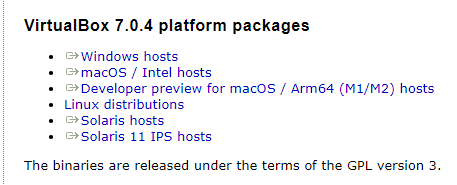
\includegraphics[scale=0.9]{Screenshot1}      	
        	\end{center}
				
			\item Klik dua kali file \textbf{VirtualBox} yang telah diinstal, lalu klik \textbf{Next}
				
				\begin{center}
					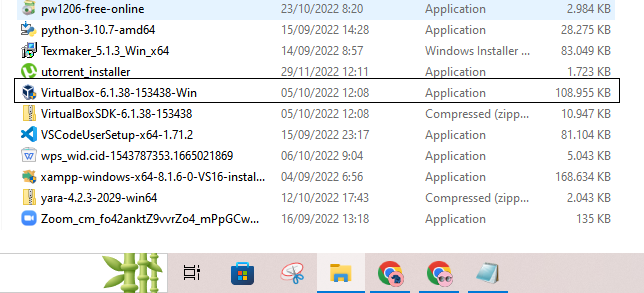
\includegraphics[scale=0.6]{Capture2.1}
					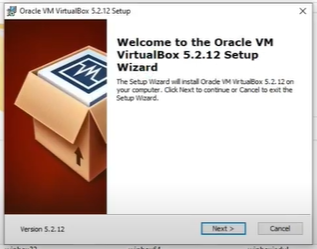
\includegraphics[scale=0.8]{Capture}	
        		\end{center}
        		
        	\item kemudian klik \textbf{Next}
        		
        		\begin{center}
        			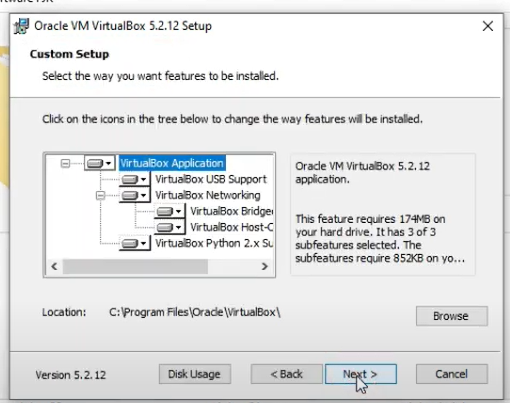
\includegraphics[scale=0.7]{Screenshot (253)}
        		\end{center}

        		
        	\item Pastikan semuanya tercentang kemudian klik \textbf{Next $>$ Yes}

				\begin{center}
					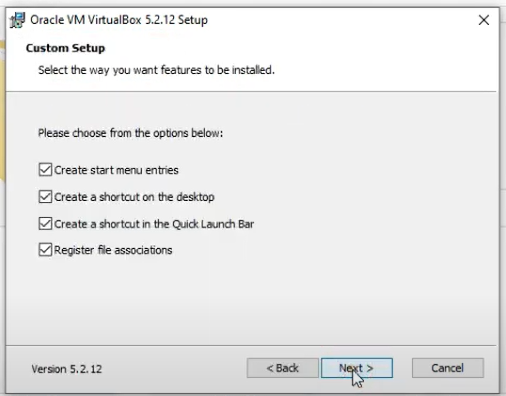
\includegraphics[scale=0.7]{Screenshot (254)}
				\end{center}
        	
        		\begin{center}
        			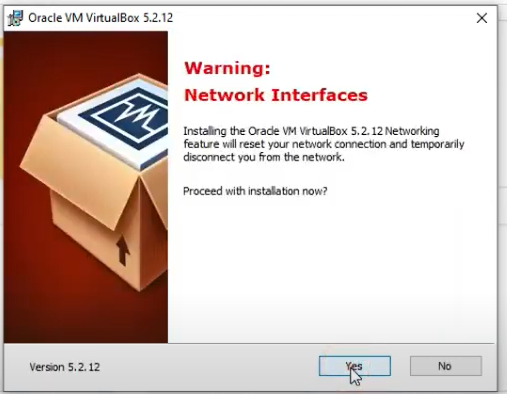
\includegraphics[scale=0.7]{Screenshot (255)} 
        		\end{center}
        		
        	\item Tunggu hingga proses instalasi selesai, kemudian klik \textbf{Finish}
        		
        		\begin{center}
        			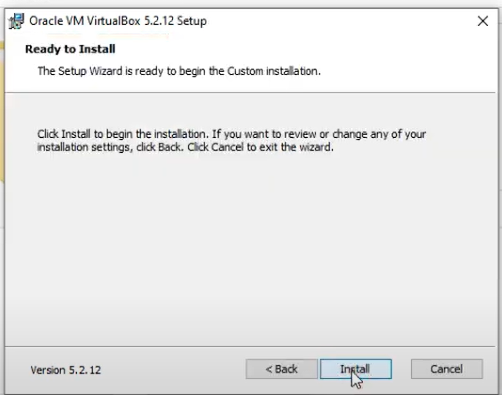
\includegraphics[scale=0.7]{Screenshot (256)} 
        			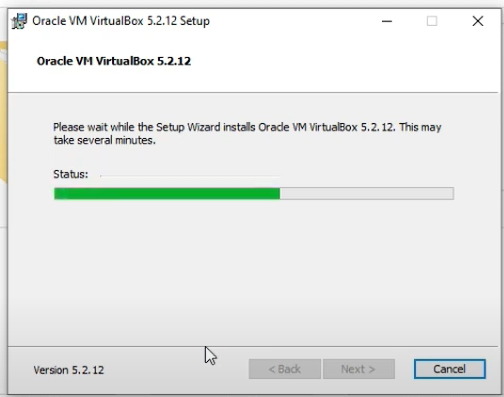
\includegraphics[scale=0.7]{Screenshot (257)} 
        			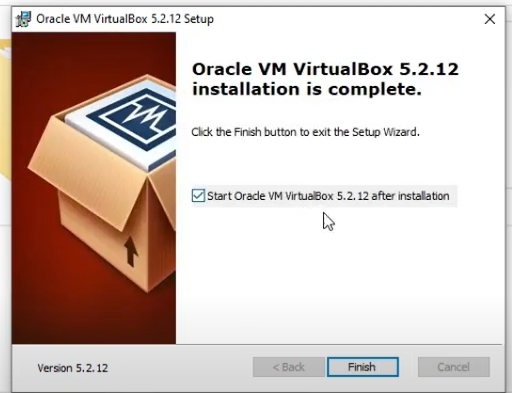
\includegraphics[scale=0.7]{Screenshot (258)} 
        		\end{center}
        		
			\item Jika tidak ada kesalahan pada saat penginstalan, tampilan \textbf{virtualbox} seperti dibawah ini akan muncul
        		
        		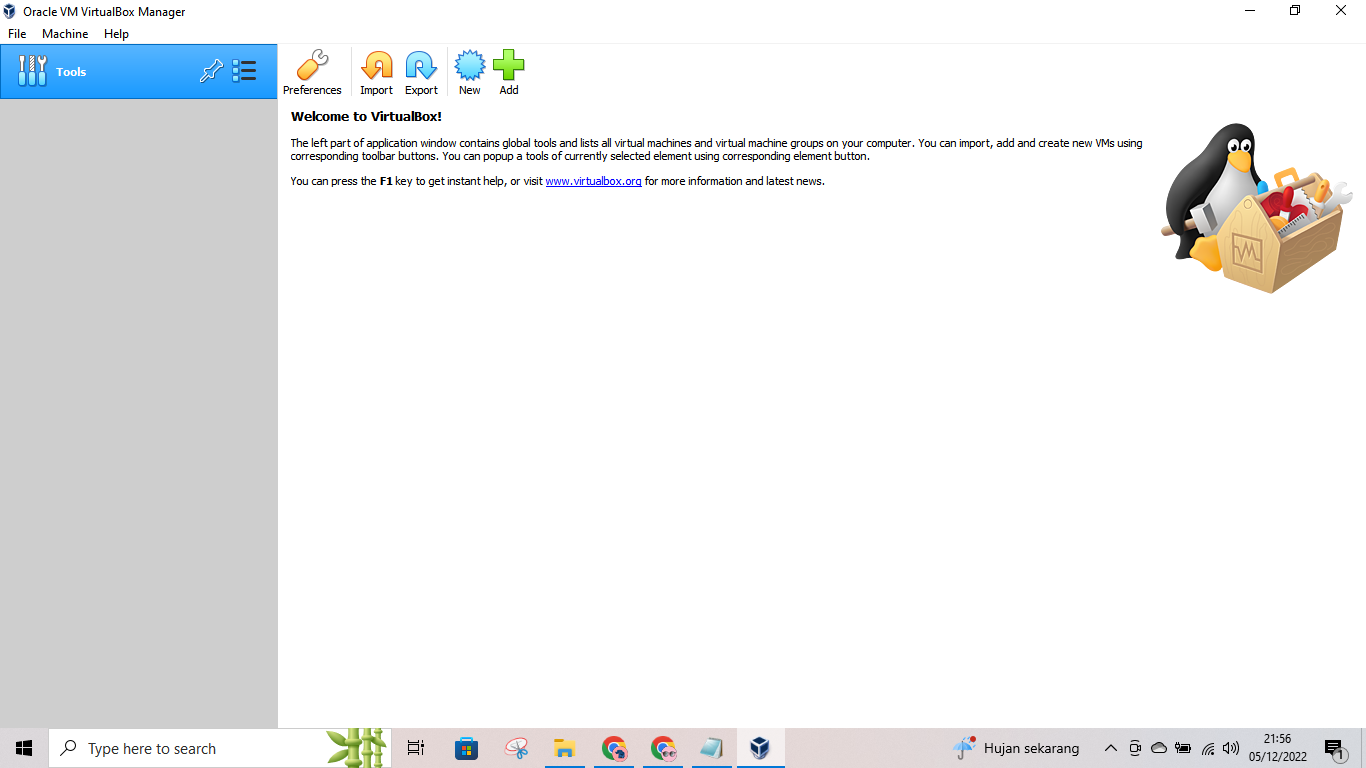
\includegraphics[scale=0.2]{vbox}        	
        \end{enumerate}

    \end{flushleft}

	\newpage
    \begin{flushleft}
        \textbf{Materi 2 -  Instalasi MikroTik pada VirtualBox}
        \newline
		\begin{enumerate}
        	\item Silahkan download MikrotikOS pada link berikut \url{https://mikrotik.com/download}
			
			\item Klik \textbf{RouterOS v6} 
			
			\begin{center}
				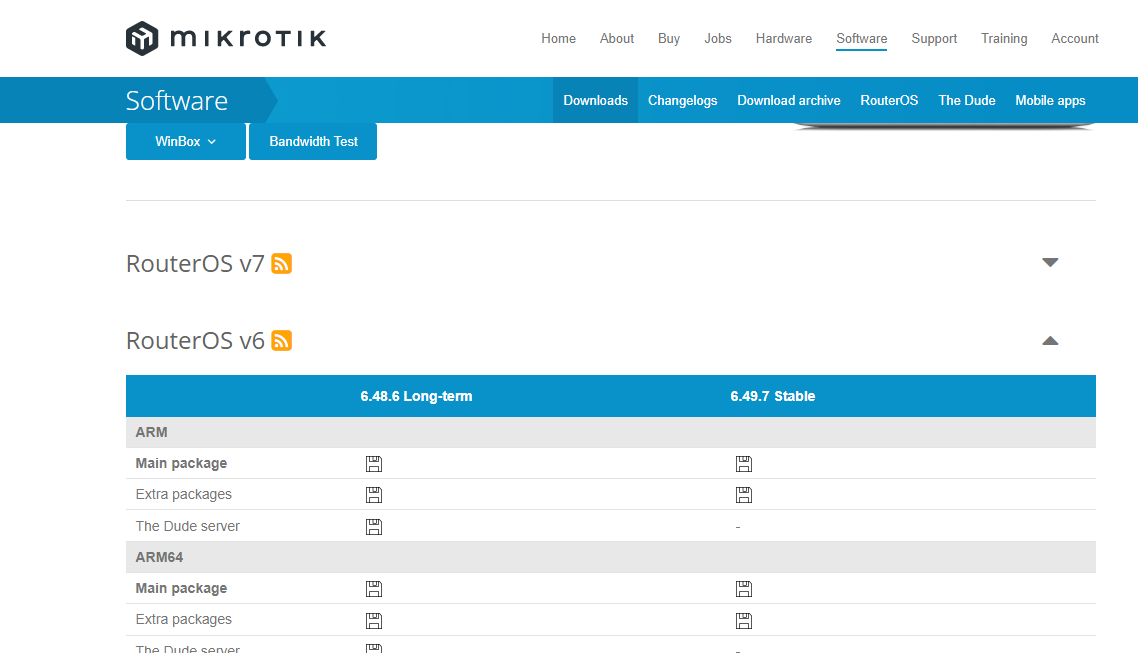
\includegraphics[scale=0.3]{routerOS}
			\end{center}
			
			\item Scroll ke bawah sampai menemukan untuk pilihan \textbf{x86}. Klik \textbf{CD image} versi stable (yang sebelah kanan). Mikrotik OS akan otomatis terdownload
			\begin{center}
				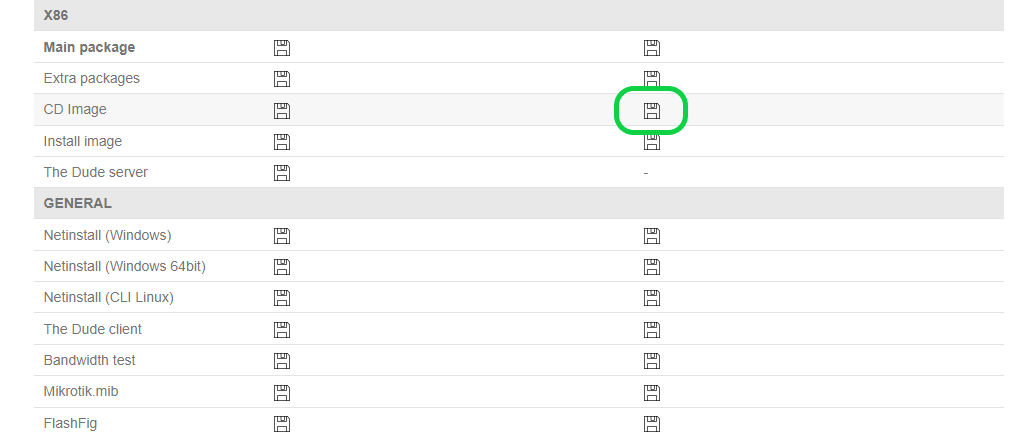
\includegraphics[scale=0.3]{routerOS2}
			\end{center}		

        	\item Klik \textbf{New}
        		\begin{center}
        			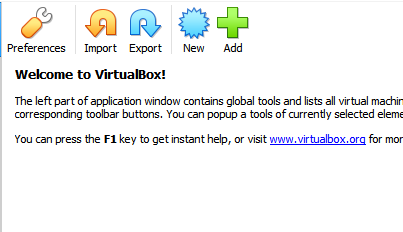
\includegraphics[scale=0.6]{virtualbox}
        		\end{center}
        		
        	\item Berikan \textbf{Name:} sesuai dengan yang kalian inginkan, atur \textbf{Type:} dan \textbf{Version:} sesuai dengan gambar dibawah
        		\begin{center}
        			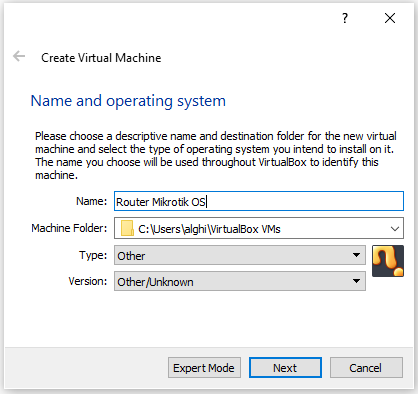
\includegraphics[scale=0.6]{(2)}
        		\end{center}
        	
        	\item Berikan ukuran \textbf{Memory size:} sebesar \textbf{64 MB}
        		\begin{center}
        			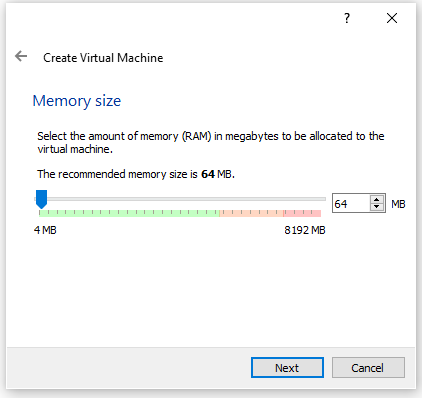
\includegraphics[scale=0.6]{(3)}
				\end{center}
				
			\item Lalu ikuti konfigurasi seperti pada gambar di bawah ini
        		\begin{center}
        			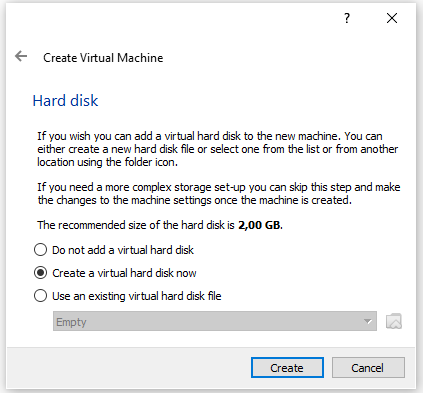
\includegraphics[scale=0.6]{(4)}
        			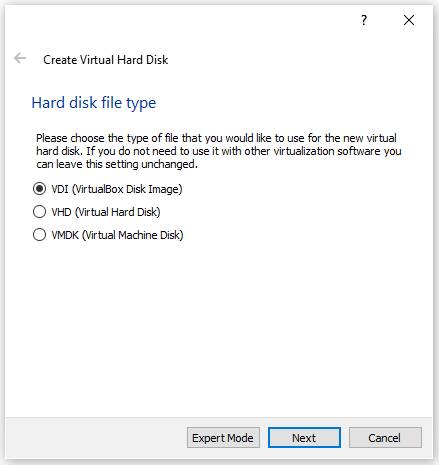
\includegraphics[scale=0.6]{(5)}  
        			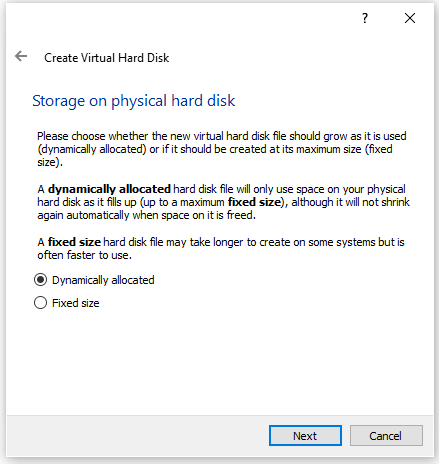
\includegraphics[scale=0.6]{(6)}
        		\end{center}
        		
        	\item Berikan ukuran penyimpanan sebesar \textbf{2,00 GB}
        		\begin{center}
        			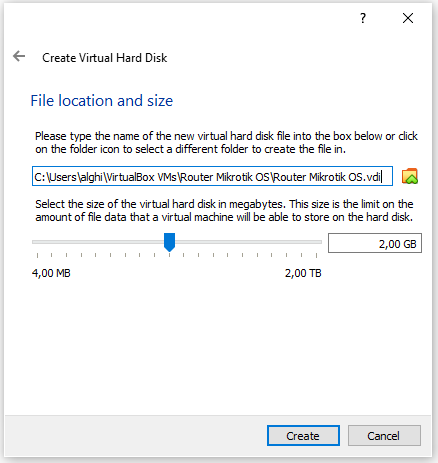
\includegraphics[scale=0.6]{(7)}
        		\end{center}
        	
        	\item Jika tidak ada error, maka akan muncul tampilan seperti dibawah
        		\begin{center}
        			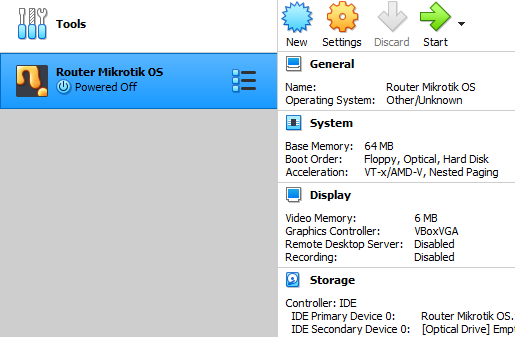
\includegraphics[scale=0.6]{terakhir}
        		\end{center}
        		        	 
        
        
        	\item Jika MiktorikOS telah berhasil di install, langkah selanjutnya adalah melakukan beberapa settingan untuk virtual machinenya
        	
			\item pastikan virtual machine yang dibuat sudah terpilih (berwarna biru), kemudian klik \textbf{Settings} 
				\begin{center}
					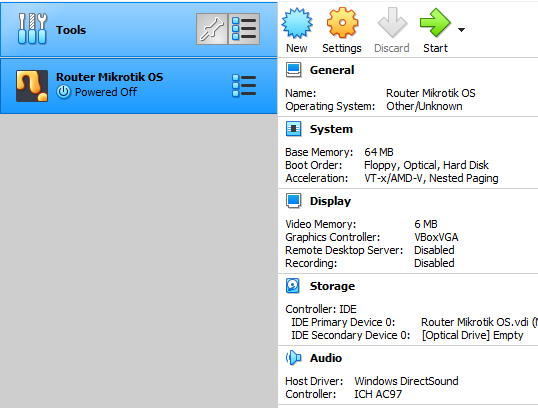
\includegraphics[scale=0.6]{(a)} 
				\end{center}
				
			\item pilih menu \textbf{Storage}, klik tulisan \textbf{Empty}, pilih menu \textbf{Choose a disk file}
				\begin{center}
					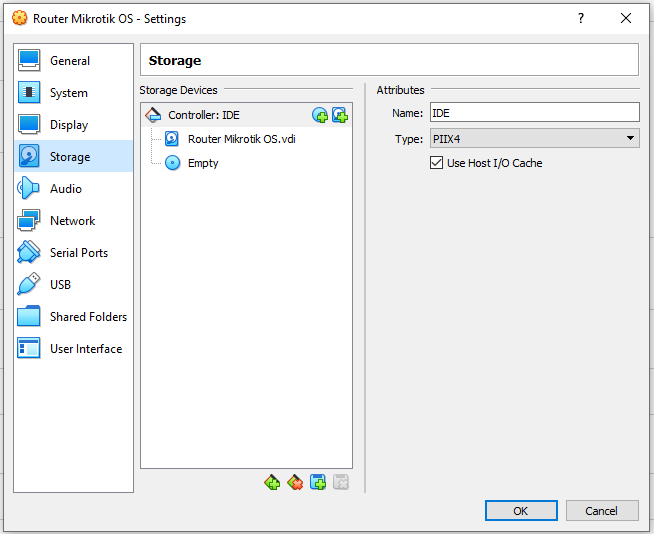
\includegraphics[scale=0.6]{(b)}
					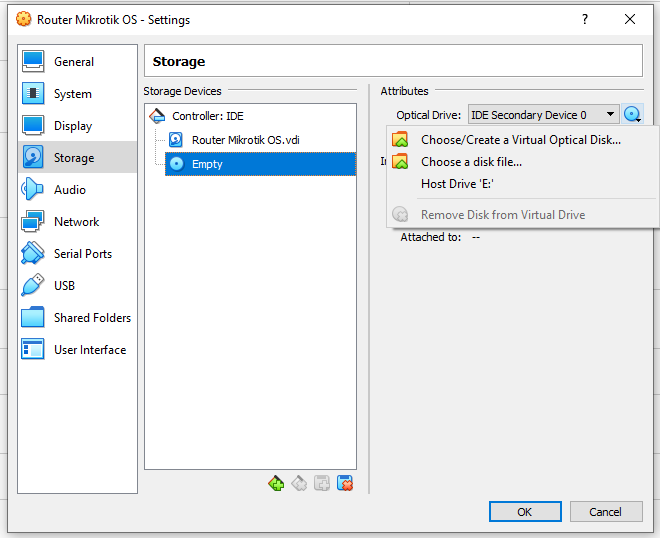
\includegraphics[scale=0.6]{(c)} 
				\end{center}
				
			\item pilih file \textbf{.iso} yang diinstall sebelumnya, kemudian klik \textbf{Open}
				\begin{center}
					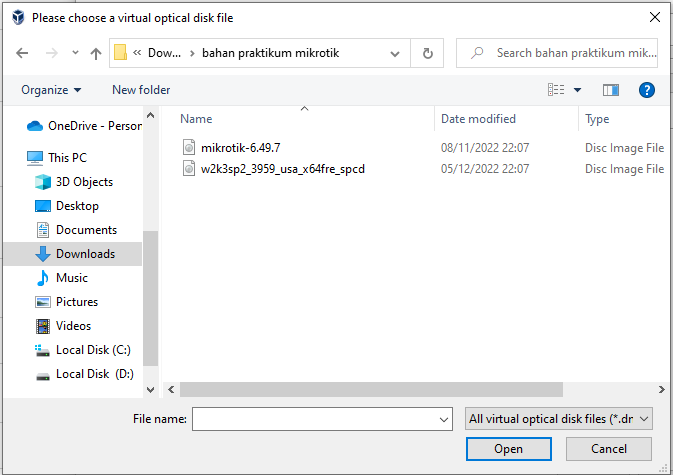
\includegraphics[scale=0.6]{(d)} 
				\end{center}
				
			\item jika sudah, maka muncul seperti dibawah 
				\begin{center}
					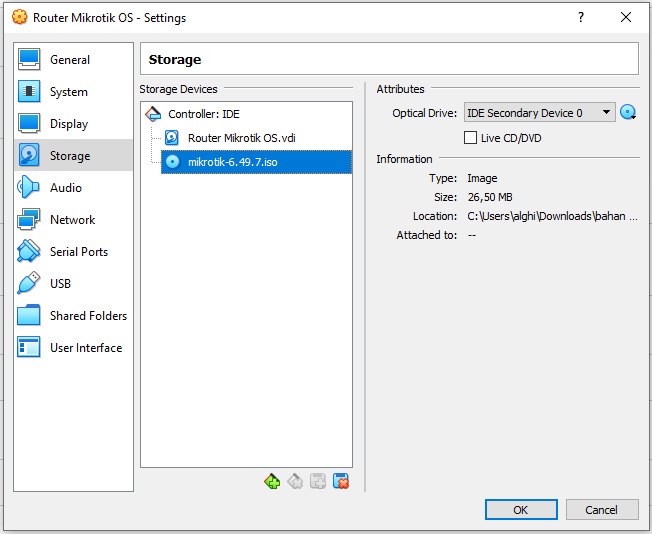
\includegraphics[scale=0.6]{(c.1)}
				\end{center}
			
			\item kemudian kita akan berpindah ke menu \textbf{System}. klik \textbf{Hard Disk} pada pilihan \textbf{Boot Order:}, klik tanda panah ke atas sampai \textbf{Hard Disk} mencapai posisi paling atas 
				\begin{center}
					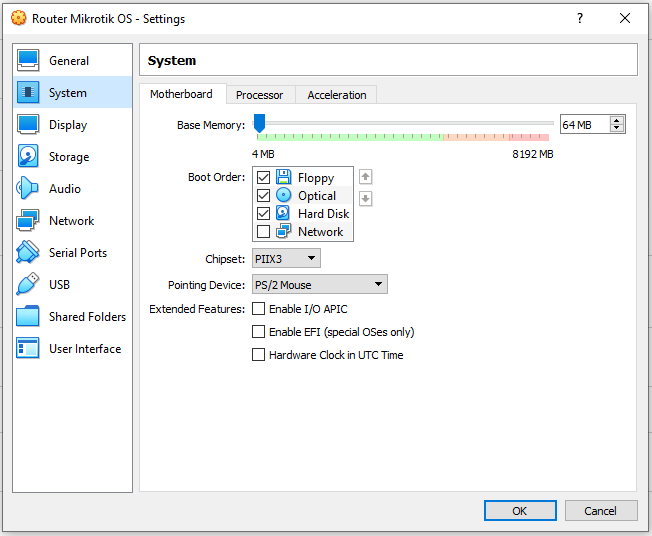
\includegraphics[scale=0.6]{(e)}
				\end{center}
			
			\item nanti akan menghasilkan hasil seperti pada gambar dibawah 
				\begin{center}
					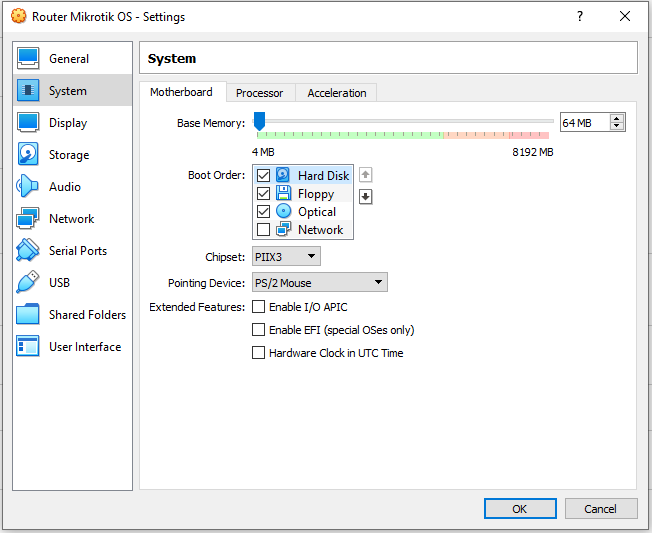
\includegraphics[scale=0.6]{(e)true}
				\end{center}
						
			\item setelah itu, klik tombol \textbf{Ok}
					        	
        	
        \end{enumerate}
		
    \end{flushleft}

    \begin{flushleft}
        \textbf{Materi 3 - Mempelajari fitur - fitur yang dapat dilakukan menggunakan Mikrotik}
        \newline

        Untuk materi lebih lanjut terkait dengan pembelajaran MikroTik
        \small\url{https://www.youtube.com/playlist?list=PLvT7-AKYOYMxXuwYv1uA9e0aDsX1XgF4l}
    \end{flushleft}

    \newpage
    \begin{flushleft}
     	\textbf{Tugas}
        \newline
        
		\begin{enumerate}
             \item Kerjakan semua langkah - langkah pada materi diatas.
        \end{enumerate}
     \end{flushleft}

 \end{document}

